%chktex-file 36
%chktex-file 23
%chktex-file 10
%chktex-file 17
%chktex-file 9
\documentclass[computationalMathematics.tex]{subfiles}

\begin{document}

%%%%%%%%%%%%%%~~~~~~~~~~~~~~~~~~~~~~~~~~~~~~~~~~~~~~~~%%%%%%%%%%%%%%%
\chapter{27th of September 2018}
\chapterauthor{A. Frangioni}
%%%%%%%%%%%%%%~~~~~~~~~~~~~~~~~~~~~~~~~~~~~~~~~~~~~~~~%%%%%%%%%%%%%%%


\begin{definition}[Minimizing sequence]
	Let $\{x_i\} \in S$ be a sequence and let $f : S \to \R^n$.
	We say that $\{x_i\}$ is a \textbf{minimizing sequence} if the sequence of function values $\{f(x_i)\}$ tends to the \emph{greatest lower bound} of $f$ ($f_* = \min \{f(x)~:x \in S\}$).
\end{definition}

\begin{example}
As an example, consider the following minimum problems and sequences:
	\[
		\min \{f(x) = x~:~x \in \R \wedge x > 0\} \text{ and the sequence } \{x_i = 1/i\} 
	\]

	\[
		\min \{1/x~:~x \in \R \wedge x > 0\} \text{ and the sequence } \{x_i = i\}
	\]
	In both cases, $\{f(x_i)\} \to 0$, but it is not an optimum.
\end{example}

\noindent We want \emph{conditions} that ensure $\{f(x_i)\} \to f_* \Rightarrow \{x_i\}\to x_* \in S \quad optimal \, solution$.

\begin{definition}[Interior and border of a set]
  Given $S \subseteq \R^n$, we say that $\vect{x} \in int(S)$ ($\vect{x}$ is an \textbf{interior point}) if it lies inside a ball contained in $S$.
  Formally, $\exists r > 0$ s.t. $\mathcal{B}(\vect{x},~r) \subseteq S$.

  Moreover, we term \textbf{border points} those $\vect{x} \in \partial(S)$ such that all the points in the ball centered in $x$ lie for a half inside the set $S$ and for the other half outside.
  Formally, $\forall r > 0~\exists \vect{y},\vect{z} \in \mathcal{B}(\vect{x},~r)$, where $\vect{y} \in S \wedge \vect{z} \notin S$.
  Intuitively, a point $x$ lies on the border if, . 
\end{definition}

Notice that a point on the boundary is not necessarily inside the ball, in that case we talk about \textbf{open set} (a set which is identical to its interior: $S = int(S)$).

\begin{definition}[Closure of a set]
  Let $S \subseteq \R^n$ we term \textbf{closure} of $S$ the set $cl(S) = int(S) \cup \partial S$.
\end{definition}

\begin{definition}[Closed set]
  We say that a set $S \subseteq \R^n$ is \textbf{closed} if it coincides with his closure: $S=cl(S)$.

  Equivalently, a set $S$ is termed \textbf{closed} if its complementary ($\R^n \setminus S$) is open.
\end{definition}

It is interesting to notice that all the functions that lead to minimizing sequences and do not converge to an optimum are all defined in open sets.

Notice that there are sets that are both open and closed, for example $\R^n$.

\begin{definition}[Bounded set]
  Let $S \subseteq \R^n$. We say that $S$ is \textbf{bounded} if $\exists r > 0$ such that $S \subseteq \mathcal{B}(0,r)$.
  
  Intuitively, a bounded set does not go to $\infty$.
\end{definition}

\begin{definition}[Compact set]
 Let $S \subseteq \R^n$. We term $S$ \textbf{compact} if it is both closed and bounded.
\end{definition}

\begin{definition}[Accumulation point]
  Let $\{x_i\} \subseteq S$ be a sequence. We say that $x$ is an \textbf{accumulation point} if $\exists~\{x_{n_i}\}$ subsequence of $\{x_i\}$ converging to $x$.
  Formally, $\{x_{n_i}\} \to x$ or $\liminf\limits_{i \to \infty} d(x_i,~x) = 0$.
\end{definition}

\begin{theorem}[Bolzano-Weierstrass]
	Let $\{x_i\} \subseteq S$ be a \emph{bounded}, \emph{real} sequence.
	Then it has a converging subsequence.	
\end{theorem}

\begin{proposition}
  Let $S$ be a compact set and let $\{x_i\} \subseteq S$ be a minimizing sequence for the objective function $f$. 
  The limit of the sequence is a feasible solution.
\end{proposition}

\begin{proof}
	According to Bolzano-Weierstrass theorem $\{x_i\}$ has an accumulation point $x \in S$.
	Since it is minimizing $f(x)$ is feasible.
\end{proof}

Why did we say \emph{feasible} but not \emph{optimal}? If the function is not continuous (cfr. \Cref{fig:27set0}) it may happen that the sequence is minimizing, but the limit is not the optimum.

\addpic{0.5}{pics/27set/1.png}{Case of non-continuity of the objective function in the border point $(0, 0)$.}{fig:27set0}

\begin{definition}[Domain]
Let $f : D \to \R$. We term $D$ \textbf{domain} of $f$ and denote $D = \text{dom}(f)$.
\end{definition}

\noindent In this course we will not take into account the domain of functions, because we can force all functions to be defined in the whole space as follows:

$f : \R^n \to \bar{\R}$, where $f(x) = \infty$ for $x \notin D$.

\begin{definition}[Graph and epigraph]
  Let $f: \R^n \to \R$. We term \textbf{graph} $\text{gr}(f) = \{(f(\vect{x}),~\vect{x})~:~\vect{x} \in \text{dom}(f)\}$.

  Conversely, we term \textbf{epigraph} $\text{epi}(f) = \{(v,~\vect{x})~:~\vect{x} \in \text{dom}(f)~\wedge~v \geq f(\vect{x})\}$, see \Cref{fig:27set1}.
\end{definition}

\begin{figure}[htb]
	\centering
	\subfigure[Graph]{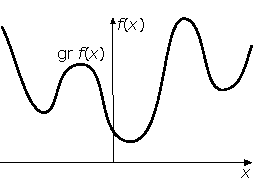
\includegraphics[width=0.35\textwidth]{pics/27set/f2.pdf}\label{subfig:27sett_graph}}
	\hspace{0.5cm}
	\subfigure[Epigraph]{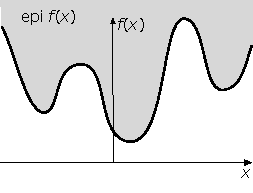
\includegraphics[width=0.35\textwidth]{pics/27set/f3.pdf}\label{subfig:27sett_epi}}\\
	\caption{Graph and epigraph}
	\label{fig:27sett1}
\end{figure}

When dealing with multidimensional inputs spaces it is crucial to have mathematical tools that make possible to somehow ``see'' the function's behaviour in a lower-dimensional space.

\begin{definition}[Level and sublevel set]
  Let $f: \R^n \to \R$.
  We term \textbf{level set} the set of all the inputs that have the same output value.
  Formally, $L(f,v) = \{\vect{x} \in \text{dom}(f)~:~f(\vect{x}) = v\}$.

  Conversely, we term \textbf{sublevel set} the set of all the inputs which image is smaller than a finxed value $v$: $S(f,v) = \{\vect{x} \in \text{dom}(f)~:~f(\vect{x}) \leq v\}$, see \Cref{fig:27sett2}.
\end{definition}

\begin{figure}[htb]
	\centering
	\subfigure[Level set]{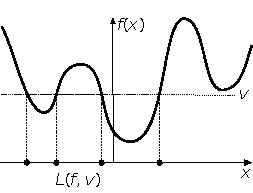
\includegraphics[width=0.35\textwidth]{pics/27set/f4.pdf}\label{subfig:27sett_level}}
	\hspace{0.5cm}
	\subfigure[Sub-level set]{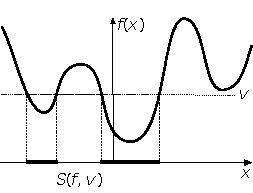
\includegraphics[width=0.35\textwidth]{pics/27set/f5.pdf}\label{subfig:27sett_sub}}\\
	\caption{Level and sub-level sets}
	\label{fig:27sett2}
\end{figure}

\section{Continuity}

\begin{definition}[Continuity]
  Let $f: \R^n \to \R$.
  We say that $f$ is \textbf{continuous} in $\vect{x}$ if $\forall \varepsilon > 0 \;  \exists \, \delta > 0$ such that $\forall y \in \mathcal{B}(x ,~\delta) ~ \abs{f(y) - f(x)} < \eps$.
\end{definition}

\begin{property}
Let $f, g: \R^n \to \R$. The following holds:

\begin{enumerate}
  \item $f+g$, $f \cdot g$ continuous at $\vect{x}$
  \item $\max\{f,~g\}$ and $\min\{f,~g\}$ continuous at $\vect{x}$
  \item $f \circ g$ $\equiv$ $f(g(\cdot))$ continuous at $\vect{x}$
\end{enumerate}
\end{property}

\begin{theorem}[Intermediate value]
Let $f : \R \to \R$. $f$ is continuous on  $[a,~b]$ if $\forall v \in \R$ s.t. $\min \{f(a),~f(b)\} \leq v \leq \max \{f(a),~f(b)\}~\exists~c \in [a,~b]$: $f(c) = v$.
\end{theorem}

\begin{theorem}[Weierstrass extreme value theorem]
Let $S \subseteq \R^n$ be a compact set and let $f$ be continuous on $S$. Then $(P)$ has an optimal solution.

Equivalently, let $S \subseteq \R^n$ compact and let $f$ continuous on $S$. Then all accumulation points of any minimizing sequence are optima and \emph{there is at least one}.
\end{theorem}

\begin{definition}[Lipshitz continuity]
Let $f: \R^n \to \R$. We term $f$ \textbf{Lipschitz continuous} (L.c.) on $S \subseteq \R^n$ if $\exists L > 0$ such that
       \[
         \abs{f(\vect{x}) - f(\vect{y})} \leq L \norm{\vect{x} - \vect{y}}~ \forall \vect{x}, \vect{y} \in S
       \]
More generally, $f$ is \textbf{globally Lipshitz continuous} if $S = \R^n$ and it is \textbf{locally Lipshitz continuous} at $\vect{x}$ if $\exists~\varepsilon > 0 ~S = \mathcal{B}(\vect{x},~\varepsilon)$. 
\end{definition}

\noindent Notice that Lipshitz continuity offers a stronger form of continuity and that the $L$ constant value depends on $S$. The wider the set the smaller $L$.

\begin{proposition}
Let $f: \R^n \to \R$.
On a compact set $S \subseteq \R^n$ if $f$ is continuous then it is Lipshitz continuous.
\end{proposition}

\begin{definition}[Lower(upper) semi-continuity]
	Let $\{\vect{x_i}\}\subseteq \R^n$ be a sequence with accumulation point in $\vect{x}$ and let $f: \R^n \to \R$.
	$f$ is \textbf{lower} (\textbf{upper}) \textbf{semi-continuous} (l.(u.)s.c.) at $\vect{x}$ if $f(\vect{x}) \leq \liminf\limits_{i \to \infty} f(\vect{x_i})$ ($f(\vect{x}) \geq \limsup\limits_{i \to \infty} f(\vect{x_i})$).

	Equivalently, $\liminf\limits{\vect{y} \to \vect{x}} f(\vect{y}) \geq f(\vect{x})$, $\limsup\limits_{\vect{y} \to \vect{x}} f(\vect{y}) \leq f(\vect{x})$.\\
\end{definition}

\section{Derivatives}

In this section we address the problem of inferring information on a complicated function around a certain value $\bar{x}$ using very simple functions, that are able to provide reliable information  around that $\bar{x}$.
Those functions are called ``derivatives''.

\noindent Let us start with a brief recap on single-dimension differentiability.

\begin{definition}[Left and right derivative]
  Let $f: \R \to \R$. We term \textbf{left derivative} $f'_{-}(x) = \lim\limits_{t \to 0_{-}} [f(x + t) - f(x)] / t$.
  
  Conversely, \textbf{right derivative} $f'_{+}(x) = \lim\limits_{t \to 0_{+}} [f(x + t) - f(x)] / t$.
\end{definition}

\begin{definition}[Differentiable]
  Let $f:\R \to \R$. We say that $f$ is \textbf{differentiable} at $x \in dom(f)$ if both left and right derivatives exist and coincide.
  Formally, $\exists f'_-, f'_+$ and $f'_-(x) = f'_+(x)$.
\end{definition}

\begin{proposition}
  Let $f: \R \to \R$ and differentiable in $x \in dom(f)$ then $f$ is continuous in $x$. 
\end{proposition}


\begin{theorem}[Mean value theorem]
Let $f : \R \to \R$ continuous on $[a, b]$ and differentiable on $(a,b)$ then $\exists \, c \in (a, b)$ s.t. $f'(c) = ( \, f(b) - f(a) \, ) / (b - a)$.
\end{theorem}

\begin{theorem}[Rolle's theorem]
Let $f: \R \to \R$. If $f(a) = f(b)$ then $\exists~c \in (a, b)$ s.t.~$f'(c) = 0$
\end{theorem}

\begin{corollary}
In the same hypothesis of Rolle's theorem, let $a$ and $b$ consecutive roots of $f$. Then $f'(a)$ and $f'(b)$ have opposite sign.
\end{corollary}

\subsection{Multivariate differentiability}

\begin{definition}[Partial derivative]
Let $f : \R^n \to \R$. We term \textbf{partial derivative} of $f$ w.r.t.~$x_i$ at $\vect{x} \in \R^n$ as
  \[
  \frac{\partial f}{\partial x_i}(\vect{x}) = \lim_{t \to 0} \frac{f(x_1,~, \ldots,~x_{i-1},~x_i + t,~x_{i+1},~\ldots,~x_n) - f(\vect{x})}{t}
  \]
       
In other words, it is just $f'(x_1,\dots,x_{i-1},x,x_{i+1},\dots,x_n$), considering each component $x_j$ where $j \neq i$ as constant.
\end{definition}

\begin{definition}[Gradient]
Given $f : \R^n \to \R$. We term \textbf{gradient} of $f$ the vector of all the partial derivatives and we denote $\R^n \ni \nabla f = \tr{(\parder{f}{x_1}, \ldots, \parder{f}{x_n})}$.
\end{definition}

\noindent The gradient is the direction on which the function increases more rapidly, while the opposite of the gradient suggests the direction on which the function decreases most.

\begin{definition}[Directional derivative]
  Let $f : \R^n \to \R$. We term \textbf{directional derivative} of $f$ in point $\vect{x} \in dom(f)$ along direction $\vect{d} \in \R^n$
  \[
    \frac{\partial f}{\partial \vect{d}}(x) :=	\lim_{t \to 0} \frac{f(x + td ) - f(x)}{t}
  \]
\end{definition}

\noindent Notice that in a multivariate space it is not possible to assure differentiability checking if the directional derivatives are equal, because there is an infinite number of different directions.

Let us now introduce the notion of multivariate differentiability.

\begin{definition}[Differentiable]
Let $f: \R^n \to \R$. We say that $f$ is \textbf{differentiable} at $\vect{x} \in \R^n$ if $\exists$ a linear function $\phi(h) = \ps{c}{h} + f(x)$ s.t.
  \[
    \lim_{\norm{h} \to 0} \frac{\norm{f(x + h) - \phi(h)}}{\norm{h}}= 0
  \]
  The intuition here is that the linear function should approximate $f$ pretty well around $x$.
\end{definition}



\begin{proposition}
Let $f : \R^n \to \R$ differentiable at $\vect{x}$. Then $f$ is locally Lipschitz continuous at $\vect{x}$.
\end{proposition}

\begin{corollary}
Let $f : \R^n \to \R$ differentiable at $\vect{x}$. Then $f$ is continuous at $\vect{x}$.
\end{corollary}

\noindent Notice that the converse does not hold.

\begin{proposition}\label{prop:27set1}
Let $f : \R^n \to \R$, let $\vect{x} \in \R^n$ and let us assume $\exists \delta > 0$ s.t.~$\forall i~\frac{\partial f}{\partial x_i}(\vect{y})$ is continuous $\forall \vect{y} \in \mathcal{B}(\vect{x}, \delta)$.

Then $f$ differentiable at point $\vect{x}$.
\end{proposition}

\noindent Notice that the converse of \Cref{prop:27set1} does not hold either.

We are now ready to introduce a class of functions that allows good results for optimization: $\C{1}$ class.

\begin{definition}[$\C{1}$ class]
	We call $\bf \C{1}$\textbf{-class} the class of functions with continuous gradient.
\end{definition}

\begin{proposition}
Let $f \in \C{1}$, then $f$ is differentiable everywhere and also continuous everywhere.
\end{proposition}

\begin{definition}[First order model]
	Let $f: \R^n \to \R$ and let $\vect{x} \in dom(f)$ We term \textbf{first order model} of $f$ at point $x$ 
	\[
	L_x(y) = \nabla f(\vect{x}) (y - \vect{x}) + f(\vect{x})
	\]
\end{definition}

\begin{proposition}
	Let $f: \R^n \to \R$ and let $x \in dom(f)$ such that $f$ is differentiable at $\vect{x}$. Then $(L_x, f(\vect{x})) \perp S(f, f(\vect{x})) \perp \nabla f(\vect{x})$.
\end{proposition}

Geometrically speaking, we can observe that a function is smooth whenever its levelsets are smooth.

\begin{example}
	Let us consider some functions that are not differentiable in the minimum.
	\begin{center}
		\begin{minipage}{0.45\textwidth}
			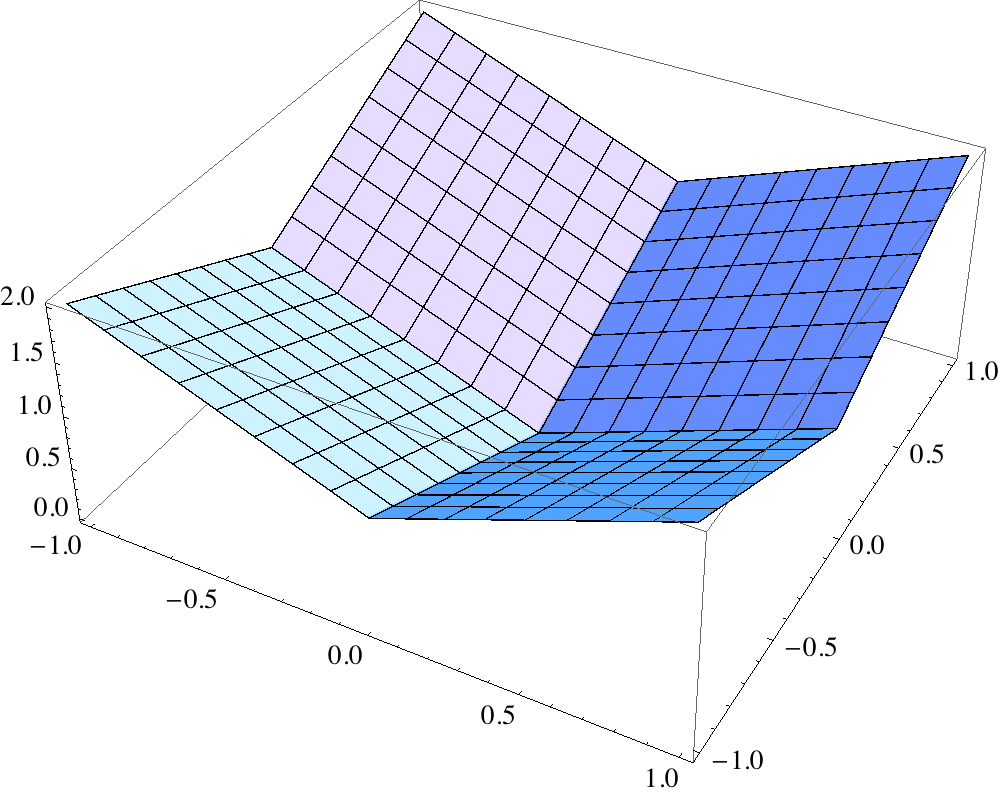
\includegraphics[width=0.8\textwidth]{pics/27set/nondiff1.png}
		\end{minipage}
		\begin{minipage}{0.45\textwidth}
			The function $f(x_1,x_2) = \norm{[x_1,x_2]} = |x_1| + |x_2|$ has some kinks.
		\end{minipage}
	
		\begin{minipage}{0.45\textwidth}
			The function $f(x_1,x_2) = \frac{{x_1}^2 x_2}{{x_1}^2 + {x_2}^2}$ may be put to $0$ in $(0, 0)$ for continuity, but it is still not differentiable in $(0, 0)$ although the function admits directional derivatives in $(0, 0)$.
		\end{minipage}
		\begin{minipage}{0.45\textwidth}
			\centering
			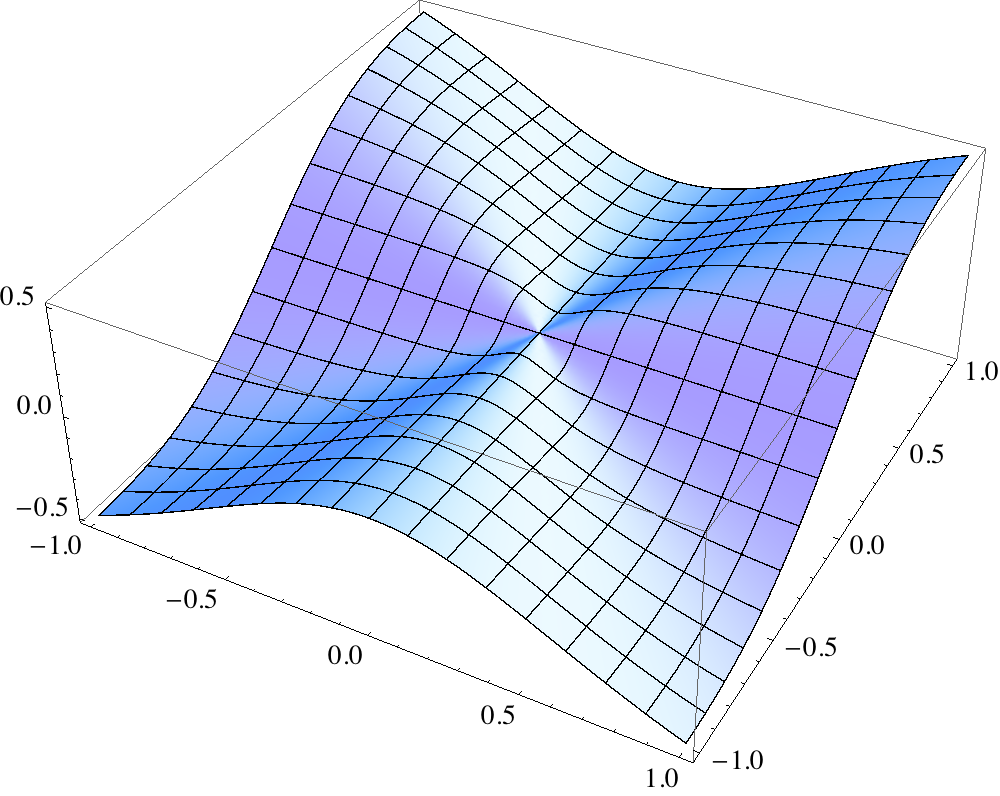
\includegraphics[width=0.8\textwidth]{pics/27set/nondiff2.png}
		\end{minipage}
	
		\begin{minipage}{0.45\textwidth}
		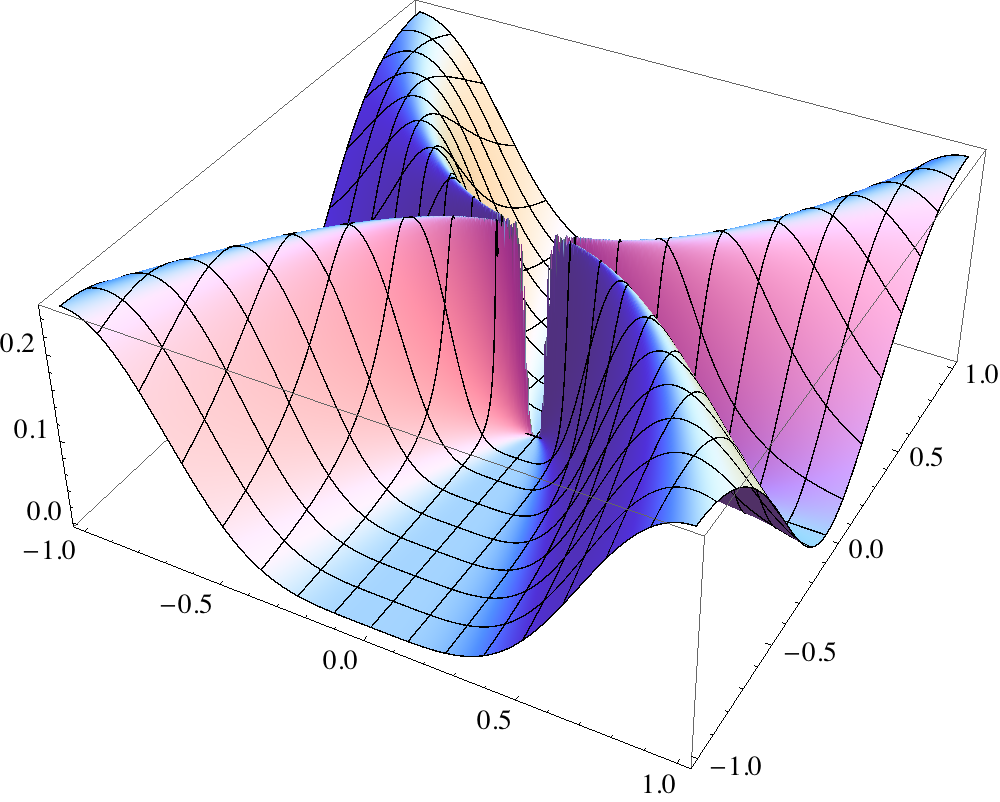
\includegraphics[width=0.8\textwidth]{pics/27set/nondiff4.png}
	\end{minipage}
	\begin{minipage}{0.45\textwidth}
		The function $f(x_1,x_2) = {\left( \frac{{x_1}^2 x_2}{{x_1}^4 + {x_2}^2} \right)}^2$ is not continuous in $0$. There are some directions that lead to the limit $0$, while there are some other directions (the parabolas above) that do not lead to value $0$.
	\end{minipage}
	\end{center}
\end{example}

\end{document}
